\section{辞書学習問題}
\begin{figure}[htb]
	\centering
	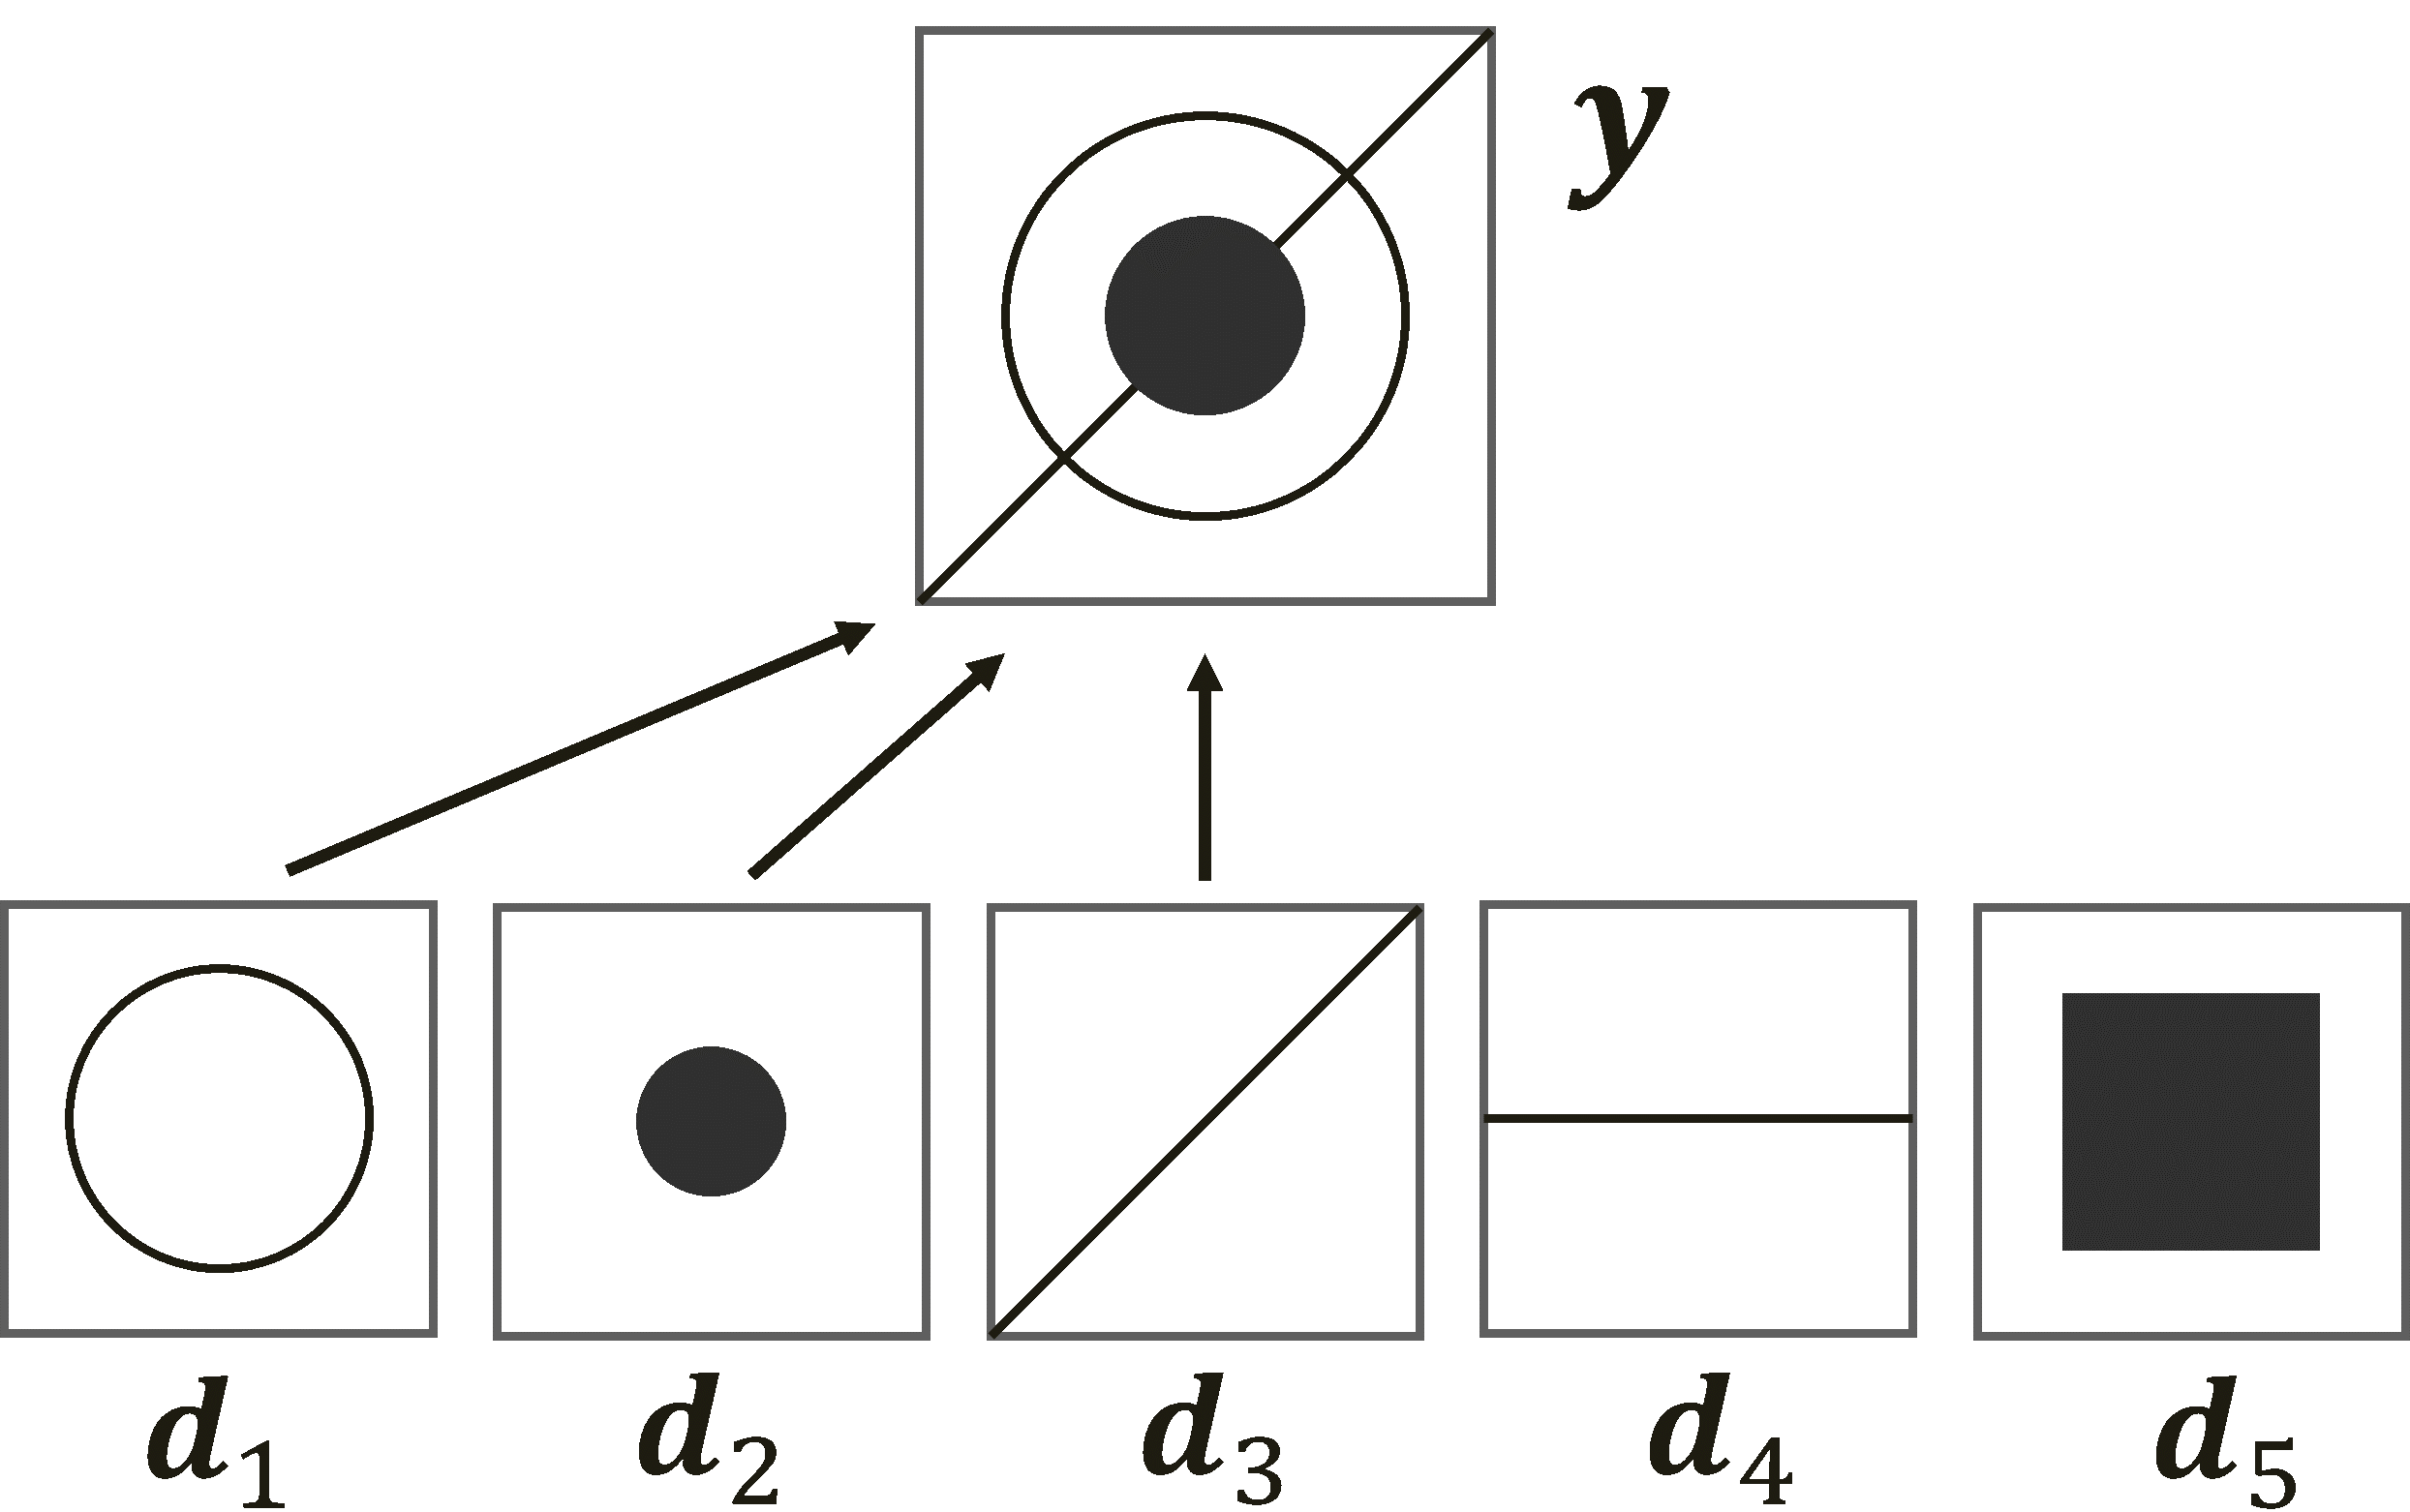
\includegraphics[width=0.7\linewidth]{image/dl}
	\caption{辞書学習のイメージ}
	\label{fig:dl}
\end{figure}

辞書学習問題では,与えられた$d$次元の信号$\bm y\in\mathbb{R}^d$ を,$K$個の辞書基底ベクトル$\bm d_i\in\mathbb{R}^d~(i=1,...,K)$と,疎な係数$\bm x_j\in\mathbb{R}^K$の線形結合で表現する問題であり,以下の最適化問題で記述される.
\begin{equation}
	D_{\text{opt}},\bm x_{\text{opt}}=\arg\min_{D, \bm x}\frac{1}{2}\|\bm y-D\bm x\|_2^2+\lambda\|\bm x\|_1~~~\text{s.t.}~~~\|\bm d_i\|_2\leq 1
	\label{dict-learn}
\end{equation}
ここで,$D=[\bm d_1,...,\bm d_K]$ であり,パラメータ$\lambda$はデータの再現精度と係数の疎性を調節するパラメータである.
問題(\ref{dict-learn})は,2変数の最適化問題であるが一般に$D$の最適化問題(辞書更新),$\bm x$の最適化問題(係数推定)に分割され,それらを繰り返し交互に解くことで解を得る.
画像処理における辞書学習問題の応用では,入力画像を小領域のパッチに分割して処理することが多い.
そのため,パッチ分割によるブロックノイズやエイリアジングが生じることがある.

\section{畳み込み辞書学習問題}
\begin{figure}[htb]
	\centering
	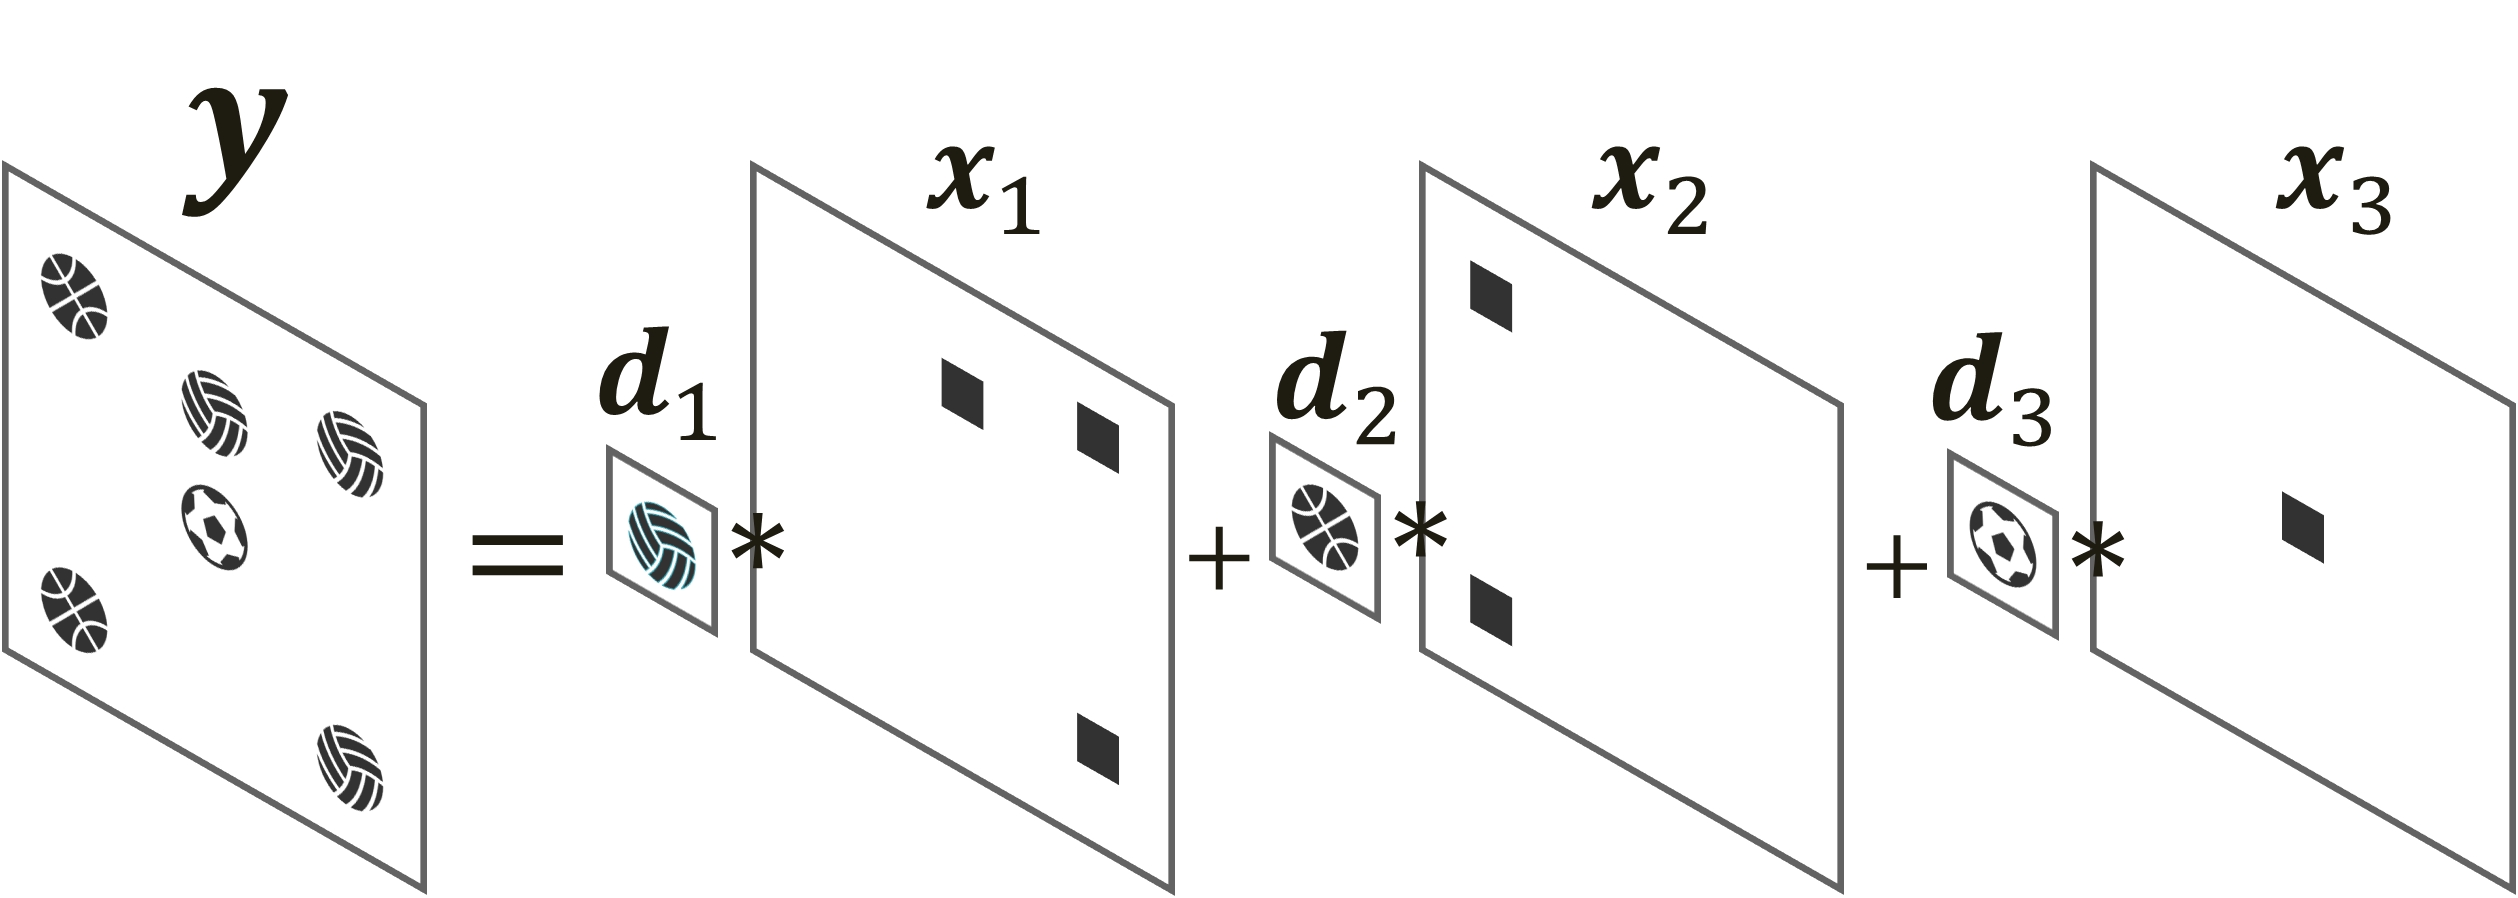
\includegraphics[width=0.7\linewidth]{image/cdl}
	\caption{畳み込み辞書学習のイメージ}
	\label{fig:cdl}
\end{figure}

畳み込み辞書学習では,与えられたサイズが$H\times W$の入力画像$\bm y\in\mathbb{R}^{H\times W}$を,サイズが$h\times w$の$K$個のフィルタ$\bm d_i\in\mathbb{R}^{h\times w}(i=1,...,K)$と,入力画像と同じサイズの$K$個の疎な係数マップの畳み込み和で表現する問題であり,以下の最適化問題で記述される.
\begin{equation}
	D_{\text{opt}},X_{\text{opt}}=\arg\min_{\bm d_i,\bm x_i}\frac{1}{2}\left\|\bm y-\sum_{i=1}^{K}\bm d_i*\bm x_i\right\|_2^2+\lambda\sum_{i=1}^{K}\|\bm x_i\|_1~~\text{s.t.}~~\bm d_i\in C_d,\bm x_i\in C_x
	\label{cdict-learn}
\end{equation}
ここで,$D=[\bm d_1, ..., \bm d_K]\in\mathbb{R}^{h\times w\times K}, X=[\bm x_1,...,\bm x_K]\in\mathbb{R}^{H\times W\times K}$ であり,$*$は巡回畳み込みを示す.
パラメータ$\lambda$はデータの再現精度と係数マップの疎性を調節するパラメータである.
$C_d, C_x$はそれぞれ,フィルタと係数マップに対する凸制約集合で,$D_{\text{opt}},X_{\text{opt}}$は問題の最適値であることを示す.
問題(\ref{cdict-learn})は,2変数の最適化問題であるため,以下に示す各変数についての最適化問題に分割する.
\begin{equation}
	D_{\text{opt}} = \arg\min_{\bm d_i}\frac{1}{2}\left\|\bm y-\sum_{i=1}^{K}\bm d_i*\bm x_i\right\|_2^2~~\text{s.t.}~~\bm d_i\in C_d
	\label{D-update}
\end{equation}
\begin{equation}
	X_{\text{opt}}=\arg\min_{\bm x_i}\frac{1}{2}\left\|\bm y-\sum_{i=1}^{K}\bm d_i*\bm x_i\right\|_2^2+\lambda\sum_{i=1}^{K}\|\bm x_i\|_1~~\text{s.t.}~~\bm x_i\in C_x
\label{x-update}
\end{equation}
問題(\ref{D-update})(\ref{x-update})を,辞書更新および係数推定の問題であり,どちらも凸最適化問題で定式化される.
両問題ともに凸計画問題の反復解法である交互方向乗数法(Alternating Direction Method of Multipliers: ADMM)\cite{admm}によって解かれ,各問題を交互に繰り返し解くことで所望の解を得る.